\documentclass{article}

\RequirePackage[svgnames]{xcolor}
\definecolor{UTorange}{RGB}{207, 83, 0} 
\definecolor{UTwhite}{RGB}{214, 210, 196}
\definecolor{UTgray}{RGB}{51, 63, 72}

\definecolor{UCLAblue}{RGB}{39, 116, 174} 
\definecolor{UCLAdark}{RGB}{0, 59, 92}
\definecolor{UCLAlight}{RGB}{218, 235, 254}
\definecolor{UCLAgold}{RGB}{255, 209, 0}

\definecolor{mered}{HTML}{882255}
\definecolor{megreen}{HTML}{004953}
\definecolor{mepink}{HTML}{AA4499}
\definecolor{rosequartz}{HTML}{F7CAC9}
\definecolor{serenity}{HTML}{92A8D1}

\definecolor{dark-red}{rgb}{0.4,0.15,0.15}
\definecolor{dark-blue}{rgb}{0.15,0.15,0.4}
\definecolor{medium-blue}{rgb}{0,0,0.5}

\usepackage{amsmath,amssymb, enumerate, tikz-cd,mathrsfs,hyperref,colortbl,bm}
\usepackage{graphicx, animate,lmodern}
\usepackage[export]{adjustbox}
\usepackage{cleveref}

\usepackage[outline]{contour}


%\usepgfplotslibrary{external}
 % \usetikzlibrary{external}
 % \tikzexternalize[prefix=tikz/]

\usepackage{float}
\usepackage{caption}
\usepackage{tikz}
\usepackage{tikz-3dplot}
\usepackage{pgfplots}
\pgfplotsset{compat=1.18}
\usetikzlibrary{scopes, angles, quotes, arrows.meta, calc, positioning, decorations.markings, decorations.pathreplacing,bending,shapes}
\usetikzlibrary{plotmarks}
\usepgfplotslibrary{colormaps}

\newcommand\fixthis[1]{\textcolor{red}{#1}}

\newcommand{\R}{\mathbb{R}}
\newcommand{\C}{\mathbb{C}}
\newcommand{\Z}{\mathbb{Z}}
\newcommand{\Q}{\mathbb{Q}}
\newcommand{\F}{\mathbb{F}}
\newcommand{\N}{\mathbb{N}}

%my macros
\newcommand{\Sphere}{\mathbb{S}}
\newcommand{\TatekG}{\mathsf{Tate}(kG)}
\newcommand{\kGMod}{kG$-$\mathsf{Mod}}
\newcommand{\StMod}{\mathsf{StMod}}
\newcommand{\Mod}{\mathsf{Mod}}
\newcommand{\Top}{\textnormal{Top}}
\newcommand{\D}{\mathcal{D}}
\newcommand{\Ho}{\mathsf{Ho}}
\newcommand{\Hom}{\textnormal{Hom}}
\newcommand{\Ext}{\textnormal{Ext}}
\newcommand{\Tor}{\textnormal{Tor}}
\newcommand{\Cell}{\mathsf{Cell}}
\newcommand{\End}{\mathsf{End}}
\newcommand{\Spec}{\textnormal{Spec}}
\newcommand{\holim}{\textnormal{holim}}
\newcommand{\hocolim}{\textnormal{hocolim}}
\newcommand{\1}{\mathds{1}}
\newcommand{\Supp}{\textnormal{Supp}}
\newcommand{\supp}{\textnormal{supp}}
\newcommand{\Pic}{\textnormal{Pic}}
\newcommand{\pic}{\mathfrak{pic}}
\newcommand{\gl}{\mathfrak{gl}}
\newcommand{\Tot}{\textnormal{Tot}}
\newcommand{\CAlg}{\textnormal{CAlg}}
\newcommand{\Res}{\textnormal{Res}}
\newcommand{\CoInd}{\textnormal{CoInd}}


\tikzstyle{vector}=[-Latex,very thick, mered,line cap=round]
\tikzstyle{xline}=[UCLAblue,very thick]
\tikzstyle{yzp}=[canvas is zy plane at x=0]
\tikzstyle{xzp}=[canvas is xz plane at y=-1]
\tikzstyle{xyp}=[canvas is xy plane at z=1]
\def\tick#1#2{\draw[thick] (#1) ++ (#2:0.12) --++ (#2-180:0.24)}
\def\N{100}


\makeatletter %for the smooth/tension example
\tikzset{
	on each segment/.style={
		decorate,
		decoration={
			show path construction,
			moveto code={},
			lineto code={
				\path [#1]
				(\tikzinputsegmentfirst) -- (\tikzinputsegmentlast);
			},
			curveto code={
				\path [#1] (\tikzinputsegmentfirst)
				.. controls
				(\tikzinputsegmentsupporta) and (\tikzinputsegmentsupportb)
				..
				(\tikzinputsegmentlast);
			},
			closepath code={
				\path [#1]
				(\tikzinputsegmentfirst) -- (\tikzinputsegmentlast);
			},
		},
	},
}
\makeatother

\pgfplotsset{
	colormap={mesvtcolor}{
		rgb255=(145,168,209) 
		rgb255=(247,202,201)
	}%,
%	colormap/mesvtcolor,
}

\pgfplotsset{
	colormap={mesvtcolorrev}{ 
		rgb255=(247,202,201)
		rgb255=(145,168,209) 
	}%,
%	colormap/mesvtcolor,
}

% mid-point rule
\pgfplotsset{
    midpoint segments/.code={\pgfmathsetmacro\midpointsegments{#1}},
    midpoint segments=3,
    midpoint/.style args={#1:#2}{
        ybar interval,
        domain=#1+((#2-#1)/\midpointsegments)/2:#2+((#2-#1)/\midpointsegments)/2,
        samples=\midpointsegments+1,
        x filter/.code=\pgfmathparse{\pgfmathresult-((#2-#1)/\midpointsegments)/2}
    }
}

% right hand sums
\pgfplotsset{
    right segments/.code={\pgfmathsetmacro\rightsegments{#1}},
    right segments=3,
    right/.style args={#1:#2}{
        ybar interval,
        domain=#1+((#2-#1)/\rightsegments):#2+((#2-#1)/\rightsegments),
        samples=\rightsegments+1,
        x filter/.code=\pgfmathparse{\pgfmathresult-((#2-#1)/\rightsegments)}
    }
}

% left hand sums
\pgfplotsset{
    left segments/.code={\pgfmathsetmacro\leftsegments{#1}},
    left segments=3,
    left/.style args={#1:#2}{
        ybar interval,
        domain=#1:#2,
        samples=\leftsegments+1,
        x filter/.code=\pgfmathparse{\pgfmathresult}
    }
}

\begin{document}

 %%Klein bottle
%         \begin{tikzpicture}
%     \begin{axis}[hide axis,
%     colormap/cool,view={-10}{30}, width=15cm, axis equal image]
%         % Draw sphere (example from the pgfplots manual)
%         \addplot3[
%             surf, z buffer=sort, colormap name=mesvtcolorrev, domain=0:180, domain y=0:360,
% 		samples=41, samples y=25, opacity=0.7,
% 		variable=\u, variable y=\v,
% 		point meta=u,
% 		] 
% 		({-2/15 * cos(u) * (
% 		    3*cos(v) - 30*sin(u) 
% 		  + 90 *cos(u)^4 * sin(u) 
% 		  - 60 *cos(u)^6 * sin(u)  
% 		  + 5 * cos(u)*cos(v) * sin(u))
% 		 },
% 		 {-1/15 * sin(u) * (3*cos(v) 
% 		  - 3*cos(u)^2 * cos(v) 
% 		  - 48 * cos(u)^4*cos(v) 
% 		  + 48*cos(u)^6 *cos(v) 
% 		  - 60 *sin(u) 
% 		  + 5*cos(u)*cos(v)*sin(u) 
% 		  - 5*cos(u)^3 * cos(v) *sin(u) 
% 		  - 80*cos(u)^5 * cos(v)*sin(u) 
% 		  + 80*cos(u)^7 * cos(v) * sin(u))
% 		 },
% 		 {2/15 * (3 + 5*cos(u) *sin(u))*sin(v)});
% 	\end{axis}
% \end{tikzpicture}


%%%%Mobius strip
%         \begin{tikzpicture}
%     \begin{axis}[hide axis,
%     colormap/cool,view={50}{35}, width=15cm, axis equal image]
%         % Draw sphere (example from the pgfplots manual)
%         \addplot3[
%             surf, z buffer=sort, colormap name=mesvtcolor, point meta=-z,  opacity=0.9,
%             samples=40, domain=-1:1, y domain=0:2*pi
%         ]
%         (
%             {(1+ x*cos(deg(y)/2))*cos(deg(y))}, % X coordinate
%             {(1+ x*cos(deg(y)/2))*sin(deg(y))}, % Y coordinate
%            sin(deg(y)/2)                           % Z (vertical) coordinate
%         );
%         \addplot3[ultra thick,
% 				UCLAblue,samples=40,
% 				domain=-1:1,
% 				y domain=0:2*pi,
% 				]
% 				(
%                 {(1+ cos(deg(y)/2))*cos(deg(y))}, % X coordinate
%                 {(1+ cos(deg(y)/2))*sin(deg(y))}, % Y coordinate
%                 sin(deg(y)/2)                           % Z (vertical) coordinate
%                 );
%     \end{axis}
% \end{tikzpicture}

	\begin{center}
		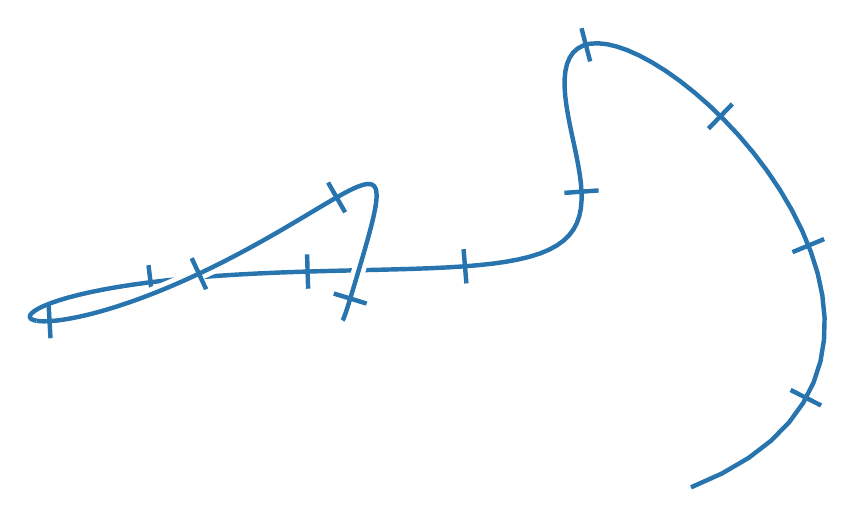
\begin{tikzpicture}[scale=2, even odd rule]
			\begin{axis}[view={65}{25},
				hide axis,
				%axis on top,
				no marks,axis equal,
				xmin=-3,xmax=3,ymin=-3,ymax=3,zmin=-1,zmax=2,
				enlargelimits={upper=0.1},
				xlabel={$x$},
				ylabel={$y$},
				zlabel={$z$}]
				\addplot3[thick,
				UCLAblue,samples=100,
				domain=0.5:2,
				y domain=0:0,
				decoration={
					markings,
					mark=between positions 0.1 and 2 step 10mm with {\arrow{Bar}}
				}, postaction=decorate
				]
				({cos(deg(2*pi*x))*e^x-1},{-sin(deg(pi*x))*e^x},{cos(deg(2*pi*x))});
				
				\addplot3[line width = 2.5pt,
				white,samples=100,
				domain=-.5:0.5,
				y domain=0:0,
				]
				({cos(deg(2*pi*x))*e^x-1},{-sin(deg(pi*x))*e^x},{cos(deg(2*pi*x))});
				
				\addplot3[thick,
				UCLAblue,samples=100,
				domain=-.5:0.5,
				y domain=0:0,
				decoration={
					markings,
					mark=between positions 0.05 and 2 step 10mm with {\arrow{Bar}}
				}, postaction=decorate
				]
				({cos(deg(2*pi*x))*e^x-1},{-sin(deg(pi*x))*e^x},{cos(deg(2*pi*x))});
				
				
			\end{axis}
		\end{tikzpicture}    
	\end{center}

 
		\begin{center}
	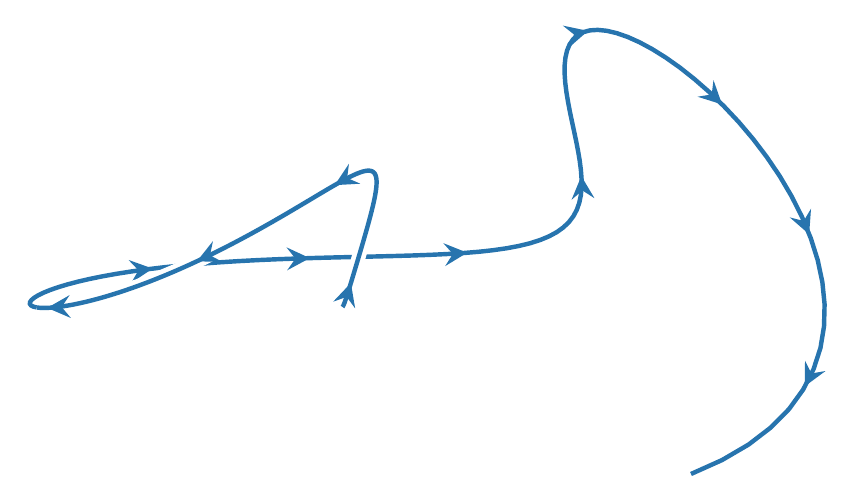
\begin{tikzpicture}[scale=2, even odd rule]
		\begin{axis}[view={65}{25},
			hide axis,
			%axis on top,
			no marks,axis equal,
			xmin=-3,xmax=3,ymin=-3,ymax=3,zmin=-1,zmax=2,
			enlargelimits={upper=0.1},
			xlabel={$x$},
			ylabel={$y$},
			zlabel={$z$}]
			\addplot3[thick,
			UCLAblue,samples=100,
			domain=0.5:2,
			y domain=0:0,
			decoration={
				markings,
				mark=between positions 0.1 and 2 step 10mm with {\arrow{stealth}}
			}, postaction=decorate
			]
			({cos(deg(2*pi*x))*e^x-1},{-sin(deg(pi*x))*e^x},{cos(deg(2*pi*x))});
			
			\addplot3[line width = 2.5pt,
			white,samples=100,
			domain=-.5:0.5,
			y domain=0:0,
			]
			({cos(deg(2*pi*x))*e^x-1},{-sin(deg(pi*x))*e^x},{cos(deg(2*pi*x))});
			
			\addplot3[thick,
			UCLAblue,samples=100,
			domain=-.5:0.5,
			y domain=0:0,
			decoration={
				markings,
				mark=between positions 0.05 and 2 step 10mm with {\arrow{stealth}}
			}, postaction=decorate
			]
			({cos(deg(2*pi*x))*e^x-1},{-sin(deg(pi*x))*e^x},{cos(deg(2*pi*x))});
			
			
		\end{axis}
	\end{tikzpicture}    
\end{center}

 
\end{document}